% !TEX root = ../../book.tex
\chapter{Trading Fundamentals}
\section{A Brief History of Stock Trading}
\subsection{Why Do we Trade}

Companies need capital to run and expand their businesses. To raise this, they can either borrow, usually paying it back over time with interest, or they can give a stake (equity) in the company to an investor in exchange for cash. As a part owner of the company the investor would then receive a portion of the profits in the form of dividends. The debt and the equity in the company,  have intrinsic value that change over time, influenced by various factors such as the success of the company, which implies higher dividends, or changes in market conditions such as changes in interest rates, returns of similar products/companies that would be compared with the return on the borrowed capital. The trading we discuss in this book simply is the act of buying and selling debt or equity (and other types of instruments) of various companies and other institutions amongst investors who have different views of their intrinsic value. The process, how trading has evolved over several hundred years makes for an incredible story of ingenuity, fierce competition and adept technology, is driven to a large extent by the positive (and sometimes not so positive) forces of money and greed. But the market designs generally lead to efficiency in evaluating the real value of a company. 


\subsection{The Origins of Equity Trading}


The first US Stock Exchange (a physical venue where trading takes place) \footnote{The first stock exchange actually dates back to 1611 in Amsterdam} the New York Stock Exchange (NYSE) was started in 1792 under a tree around Wall St in lower Manhattan when a group of 24 brokers signed the Buttonwood Agreement which bound the brokers to trade only with each other under specific rules. They soon moved into a coffee house (Tontine Coffee House) and various locations around Wall St. before settling in the current location on Broad St. in 1865 (Wikipedia citation). Over the next 100 years stock exchanges evolved in complexity and breadth but renaming conceptually unchanged the physical location where traders and stockbrokers met in person to buy and sell securities Most of the exchanges settled to a communication system named Open Outcry where new orders where communicated to the floor via hand signals and with a Market Maker facilitating the transactions often stepping in to provide short term liquidity. Telegraph and then the Telephone had big effect in accelerating the process and the dissemination of the information but not on the fundamental process in which trading was actually done. 


\subsection{Electronification and the Start of Fragmentation}


This changed in 1971 when the NASDAQ Stock Exchange was launched as a completely electronic system. Initially started as a quotation site it quickly turned into a full execution venue and the second largest US exchange by market capitalization. Things were heating up. In 1969 the Institutional Networks Corporation launched Instinet a computerized link between banks, mutual fund companies, insurance companies so that they could trade with each other with immediacy, completely bypassing the NYSE.  Instinet was the first example of an ECN (Electronic Communication Network) and alternative way of trading that grew in popularity in the 80s and 90s to include other notable ones like Archipelago and Island ECNs. This evolution started a trend in market structure that only got more accentuated over time and created significant challenges to the traditional approach to trading and accelerated the electronification of trading: Fragmentation.


\subsection{The Birth of HFT and Algorithmic Trading}


 The year 2001 brought another momentous change in market microstructure. On April 9th, 2001, the SEC mandated that the minimum price increment on any exchange should change from 1/16th of a dollar ($\approx6.25$ cents) to 1 cent. This seemingly  minor rule change with the benign name of 'Decimalization' (moving from fractions to decimal increments) had actually dramatic effect, causing the average spread to significantly decrease and with that the profits of market makers and broker dealers. Less profit meant force some market making firms to exit the business and reduced the liquidity. To bring liquidity back exchanges introduced the maker-taker fee model which would compensate, in the form of rebates, the trader that provided liquidity (makers) while charging the regular fee to the consumer of liquidity (takers)\footnote{For some readers the concepts of providing and taking liquidity might be murky at best. No fret, this will all become clear when we discuss the trading process introduce market microstructure}. This created additional unintended consequences. Now if somebody could mostly provide liquidity limiting liquidity taking, she could make a small profit with minimal risk and need for capital. This would need to be to be automated as the per trade profit would be minimal and one would have to trade a lot to generate real revenue. They would also need to be fast because position in the order book and speed of cancellation of limit orders are both critical for profitability. This led to the explosion of what today we call High Frequency Trading or HFT and to the wild technology arms race by the whole industry to become faster and faster. HFT style (what used to be called opportunistic market making) already existed but never as a significant portion of the market. At it's peak it was assumed that more than 60\% of all trading was generated by HFTs. With trading costs decreasing trading volume increased but the drop of trading commission and profitability forced broker dealer to start automating some of their more mundane trading activities. Simple workflow strategies slowly evolved into a whole field that we call now as Algorithmic Trading which is a major topic of this book.  


\subsection{Dark Pools and Reg NMS}


Over the following several years, fragmentation continued to increase and microstructure evolved further. New venues surfaced that had a different value proposition:  allow traders to find block liquidity without having it to convey that information to a block trade market maker. No market data was  published from these venues only the notification of a trade after the fact thus these venues were aptly but somewhat ominously named Dark Pools. In 2005 Regulation NMS was introduced to try to protect investors from the increase complexity and fragmentation. The core of the rules where the Order Protection or Trade Through rule that dictate are that an order submitted to any market should get the best of prices in all markets (actually a set of 'protected' markets). This forced exchanges to link to each other and broker dealer into building systems called Smart Order Routers to manage the requirements implied by the rules.


\subsection{Conclusions}


This whirlwind history of trading bring us to present times. It's not meant to be comprehensive but simply to provide the history and background that led to the dizzying complexity of modern market structure which would seem insane without the appropriate context. Europe and Asia had somewhat slower and somewhat compressed evolution but the main features are more or less similar.

The markets continue to evolve and will discuss more recent events in the next section where we provide an overview of the current state of Market Structure.


\section{Market Structure and Trading Venues: A Review}

\subsection{The Equity Markets Participants}
With all the context acquired in the previous section we can now jump in a brief review on the state of Market Structure. 

In order to get a sense of the underpinning of Equity markets  it is important to understand the the various participants in the markets, why they trade and what they care about.

\begin{itemize}
\item Long Only Asset Managers: These are the traditional Mutual Funds providers like Vanguard, Fidelity, etc where most of us invest our 401ks.  They are named Long Only because they are restricted from short selling (where you borrow shares to sell in the market in order to bet that the price drops) and can only profit through dividends and appreciation. They have several Trillions under management and need to continuously trade in order to re-balance their large portfolios so as to achieve the objective of the strategy which is to track and hopefully beat a particular benchmark. Their time horizon the care about is in general long from months to years. Historically less sophisticated in their trading operations they tend to be less concerned by transaction costs since the timescales are quite long and the returns they target dwarf the few dozen basis points incurred in trading. They tend to be very concerned and sometimes even paranoid around information leakage and fear that the "Sharks" in the market realized what their are up to and take advantage of them. 

\item Hedge Funds and Long-Short Asset Managers: A myriad of large and small firms targeted to institutional clients and wealthy investors often running  several different strategies most often Long-Short strategies in order to perform well in both raising and falling markets. They include Bridgewater, Renaissance Technologies, Point 72 (former SAC Capital), and many others.  Their time horizon is as broad as the strategies they employ but in general they are shorter than Long Only counterparts. In general they have more sophisticated traders who are really careful to minimize transaction cost since they often make many more smaller bets and TCs are a significant fraction of their profits.

\item Broker/Dealers:  They sit in between the "Buy Side' (generic term for asset management firm) and the various exchanges (note that only member firms are allowed to trade on exchange and most asset management firms are non-members). They can act either ad Agent for the client (i.e. Broker) or provide liquidity as Principal (i.e. Dealer) from their own accounts. They also historically had large proprietary trading desks investing the firm's capital using strategies not dissimilar to the ones Hedge Funds would use. Since the introduction of the Dodd-Frank Act \footnote{\url{https://en.wikipedia.org/wiki/Dodd\%E2\%80\%93Frank_Wall_Street_Reform_and_Consumer_Protection_Act}} the amount of proprietary risk that a firm can carry has dramatically decreased and most bank shed large part of it's proprietary trading activities either shutting down the desks or spinning them off in indipendent Hedge Funds.

\item HFTs and ELPs (Electronic Liquidity Providers), DMMs (Designate Market Makers): These participants generate returns by acting as facilitators between the above participants, providing liquidity and then trying to unwinding it at a profit. They can also be aggregators of retail liquidity ( e.g. individual investors trading using online provides like ETrade). Likelyu the most  and technology savy operators they leverage ultra-low-latency infrastructure to be able to be extremely nimble to get in and out of the markets and take advantages of tiny mis-pricing.

\end{itemize}

\subsection{Equity Markets Watering Holes}
Now that we know who the players are let briefly review the various approaches to liquidity access.

\subsubsection{Exchanges}

This is the default approach to trading and still account for about 60-70\% of all activity. This is where an investor will go when he's looking for immediacy and a more certain outcome. Because it's full Orderbook is public and arrival/cancellations are all broadcasted one knows exactly what liquidity is available and can plan accordingly. But that information comes at a cost as the same information is know by all participant especially (due to their often technological advantages) the ones whose strategies are looking for patterns of large directional trades  they can take advantage on. A trader that needs to buy or sell in size will need to be very careful on how much information it conveys or it might pay dearly. The field of algorithmic trading execution is the effort of trading in large sizes while minimizing the information leakage.

But apart from the leakage concerns it is the most basic approach to trading. Or It would be if it wasn't that at the time of this writing a US equity trader can buy or sell stocks  in 14 different exchanges\footnote{\url{https://www.sec.gov/fast-answers/divisionsmarketregmrexchangesshtml.html}}. These exchanges are all "protected" meaning that liquidity at the best prices cannot be ignored and exchange will need to route route to these exchanges when prices are better (charging a fee for the honor). To effectively trade on exchanges in an effective way traders required advanced technology in the form of a Smart Order Router a trading system that is able to access all the exchanges and split up and route these orders to the various exchanges to access all that liquidity \footnote{Technically broker could all send to one exchange but the costs of the exchange routing any order to access protected quotes would be exceedingly large}.

On the exchange side, recent years have seen a consolidation of many exchanges in the hands of on three main players: NYSE, NASDAQ and CBOE/BATS. Here is a list of venue operated by each:
\begin{itemize}
\item NYSE: NYSE, Arca, MKT LLC ( former AMX, American Stock Exchange), NSX (form National Stock Exchange), CHX (former Chicago Stock Exchange)
\item NASDAQ:  NASDAQ, PHLX (former Philadelphia Stock Exchange), MRX( forme ISE Mercury, ISE (former Internaltional Securities Exchange, GEMX (forme ISE Gemini), BX (former Boston Stock Exchange)
\item CBOE/BATS: CBOE, BZX ( former BATS), BYX (former BATS-Y), EDGEA, EDGEX, C2
\end{itemize}

Notable mention is the newest exchange and as of now the only independent exchange is The Investors Exchange or IEX. We'll discuss this further on in the section

The curious thing is that this consolidation did not happen with a contemporaneous reduction in fragmentation. These venues continue to operate as separate pools of liquidity. There is a simple explanation for this, although probably the above exchange will deny that. More and more exchanges revenue model is centered around market data fees, the consts it charges to broker/dealer to get access to their direct market data fees. Since the venue quotes are protected any serious operator will need to use these feeds in their trading applications and the more exchanges the more connections and fees these exchange can charge. Regulators are starting to look into this issue.

Something that is even more curious is that all the exchange are located in mainly 4 huge data centers all located in the New Jersey countryside: Mahwah, Secaucus, Carteret, Weehawken. The distance between these data centers adds some latency in the information dissemination across these exchanges creating latency arbitrage risks as super fast HFTs co-located in each data center and leveraging the best technology like microwave tower between datacenters can see market data change before others and using that information to either trade ahead or remove liquidity if they see on market move faster. 

All exchange have almost exactly the same trading mechanism and from the trading perspective behave exactly the same way during the continuous part of the trading day (i.e excluding the opening and closing auction which we will talk in a separate section). They provide a visible (meaning that market data is disseminated) order book and operate in a price/time priority basis. Most of them use the Maker-Taker fee model that we discussed in the previous section but a few: BTY, EDGA, NSX  have adopted an 'Inverted' fee model where posting liquidity incurs a fee while it provides a rebate for taking liquidity. This subtle but significant difference causes these venue behavior to be markedly different. The cost for providing liquidity would discourage HFTs from providing liquidity to collect rebates on the other side thought the rebate awarded to the taker would imply that these venues are used first creating incentives for the provider who are OK to pay to find liquidity at that price. This interplay creates subtle and still not well understood dynamics in the way the market as a whole behaves.

Finally a few words about IEX. It started as an ATS whose main innovation is a 38-mile coil of optical fiber placed in front of its trading engine that introduces a 350 microseconds each way aptly named a "speed bump" that is meant to  remove the speed advantages of HFTs. This would reducing the efficacy of their more predatory tactics and thus provide a liquidity pool that is less toxic. On June 17 2016 IEX became a fully fledged exchange after a very controversial process and with big fanfare about an exchange that would be different and would attract substantial liquidity due to it's innovative speed bump. As of 2018 this potential remains unrealized and IEX has not moved much from the 2\% market share of which 80\% is still hidden liquidity.

\subsubsection{Alternative Trading Systems/Dark Pools}

As discussed above trading in large blocks in exchanges is not a simple matter and requires advanced algorithms and smart order routers. Even with those the risk and realized costs due to information leakage can be significant. Dark Pools where invented to try to counterbalance this situation. One investor can have a large order sitting in a dark pool without anybody knowing she is there and might be able to find the other side without showing their hands. As discussed dark pools do not display any order information and uses the NBBO (National Best Bid/Offer) as their reference price. In almost all cases, to avoid having to access protected venues, these pools only trade at the inside market (at or withing the bid ask spread) although, on order to maximize the probability of finding liquidity most of the block interaction happens at the midpoint. This type of trading has gained more and more traction in the last 15 years and now accounts for 30--40\% of all traded volume. Clearly the growth of dark execution has spurred a lot of competition creating what is likely too much of a good thing. 

As of 2018 there are a 33 ATSs (Alternative Trading System) \footnote{\url{http://www.finra.org/industry/equity-ats-firms}} and N (?) Single Dealer Platforms\footnote{Internal Sources}!  All these venues compete on pricing, availability of liquidity, system performance, functionality such as special order types etc. 

Most of these ATS are run by the major investment banks. UBS's ATS, Credit Suisse's Crossfinder, Deutsche Bank's SuperX, Morgan Stanley's MS Pool and Barclyas' LX are, in order,  the top five broker pools by volume in the US with UBS leading by a large margin being almost double the volume of the 2nd most active venue. Many brokers have more than one pool to support specialized usecases(e.g Morgan Stanley has a VWAP crossing ATS). Othe venue were born out of the fundamental desire for investment firms to trade directly with each other bypassing the intermediaries and  thus reduce cost and remove information leakage. Main problem of these Buyside to Buyside approaches is that most of the trading approaches of these firms are highly correlated ( e.g. two funds tracking the same benchmark) and thus the liqudidity tends to be on the same size. So all of these venues have found different approaches to leverage Sell side broker's liquidity to supplement it. BIDS and Liquidnet  are the biggest ATSs of this type with BIDS the one that had significant growth in recent years and Liqudinet fading it's initial dominance marred by a scandal that tarnished its reputation and client confidence. 

The space is very active with new venues popping up on a regular basis with the promise that the new approach finally found the magic bullet of finding the liquidity that is needed without anybody knowing.

\subsubsection{Single Dealer Platform/Systematic Internalizers}
An increasing number of trading firms in recent years started providing direct access to their internal liquidity. Broker/Dealers and other institutional clients connect to these Single Dealer platform directly. These SPDs send regular Indication Of Interest (IOI)  that are bespoke to a particular connection and the broker can respond when there is a match. This approach is growing fast. Because SDPs are not regulated ATSs they can offer somewhat unique products. Brokers themselves are starting to provide their own SDPs to expose their internal liquidity. A quickly evolving space that promise interesting innovation but alas further complication in this already crowded ecosystem.

\subsection{Auctions}
As we will discuss in future sections primary exchanges (exchanges on which a particular instrument is listed) begin and end the day with a (primary) auction procedure that leverages special order types to accumulate supply and demand and then runs an algorithm that determines the price that would pair off the most volume. The Closing Auction is of particular importance since the many funds set their NAV (Net Asset Value) based on the official closing price. This leads traders to want to trade as close to the close as possible to optimize the dual objective of getting the best price but also deviating as little as possible from the close price. The explosive growths of ETFs (Exchange traded Funds) has exacerbated this trend in recent years and recently {TBD}\% of the total day volume trades in the last 30m. Recent months have brought a lot of movement in this area with brokers and DSPs trying to provide unique ways to expose internal liquidity marked for the closing auction.
 
\subsection{Beyond the US}
Is this situation unique to the US? Yes and no. European and Asian exchanges have operated as monopolies for a lot longer than their US counterparts and the evolution of ATS/Dark Pools and other MTFs (Multilateral Trading Facilities) have followed suit but in a more subdued manner. The trading in these markets has always been smaller and concentrated and there is not enough liquidity to support 50 different venues. Additional complexity is the very different regulatory environments in these various countries limiting cross-border trading. Today off exchange volume in EU is still limited to around {TBD}\% and even less ({TBD}\% in Asia.

\subsection{Conclusions}
Modern Market Structure can feel like a jumbled mess. It is. Fully understanding the implications of these different methods of trading tied by regulation, competition, behavioral idiosyncrasies due participants lack of understanding and influenced by perception and preconceived notions  is a likely impossible task. But it's an environment that every practitioners will have to navigate and make the best of it. Creating systematic models that can capture all these subtle difference is a futile task and the quantitative modeler in Algorithmic Trading will be forced into coarse abstractions and generalization. They will then have to be most likely enhanced by often questionable heuristics to account for the residual complexity. Market Structure is also a fascinating ecosystem continuously evolving through the forces of ingenuity, competition, and greed to make a profit providing tools and services to institutional investor in their  strive to reduce the cost of executing an investment mandate. We hope the above provides the reader with at least with a starting point in the exploration of this fascinating  experiment.


\section{The Mechanics of Trading: The Limit Order Book}


In automated continuous double auction trading system that have become prevalent in financial markets, buyers and sellers submit limit orders electronically; orders are then matched and executed as per time and price priorities.\footnote{Not all exchanges are matching orders following a Price/Time priority algorithm; a key characteristic of the Futures market, for instance, is the existence of pro-rata markets for some fixed income contracts where passive child orders receive fill from aggressive orders based on their size as a fraction of the total passive posted quantity} The unmatched orders are stored in the limit order book (LOB) awaiting further execution. Market orders are orders seeking the best available price and they are executed immediately. Thus, one way or another all executed orders can be considered as marketable orders.


In practice the state of the order book changes quite rapidly due to he multi-agent nature of financial markets and the prevalence of high frequency trading. One can consider there are six types of events, three on either side, that can alter the state of the order book:
	\begin{itemize}
	\item Limit order submission: A limit order is added to the queue at the specified price level.
	\item Limit order cancellation: An outstanding limit order is expired or cancelled and therefore is removed from the LOB.
	\item Marketable order submission: outstanding limit orders at the best price and up to the demanded liquidity price level (in case of pure market order) or up to the limit price (for marketable limit order) are executed against the incoming order and thus removed from the book.
	\end{itemize}


Orders on the buy side are called ``bids'' while those on the sell side are called ``asks.'' The above events are illustrated in Figure~\ref{fig:limbk1} to Figure~\ref{fig:limbk3}. \\
	\begin{figure}[!ht]
	   \centering
	   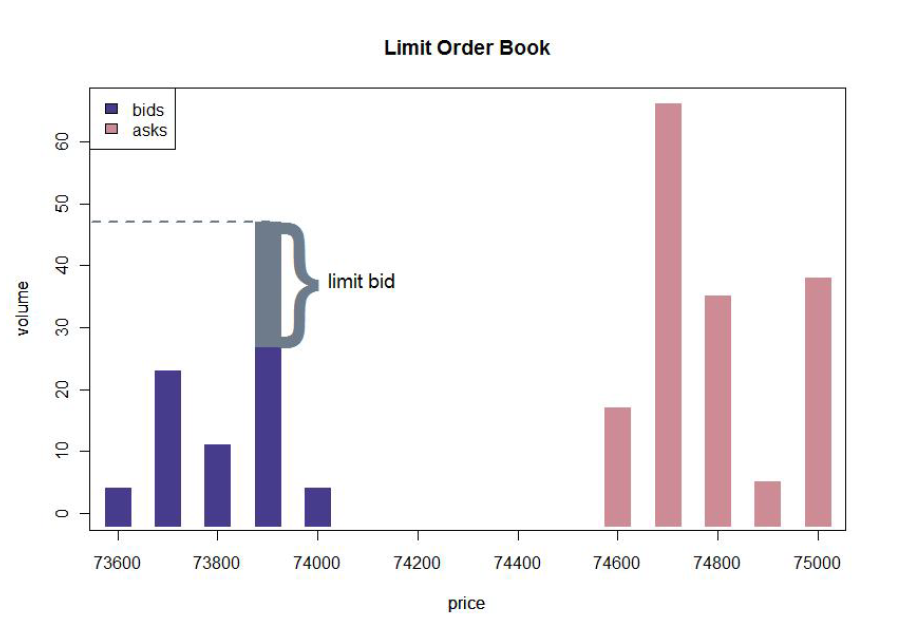
\includegraphics[width=0.9\textwidth]{chapters/chapter_trading_fund/figures/limitbk1.png} 
	   \caption{Limit Order Book---Limit Bid. \label{fig:limbk1}}
	\end{figure}
	\begin{figure}[!ht]
	   \centering
	   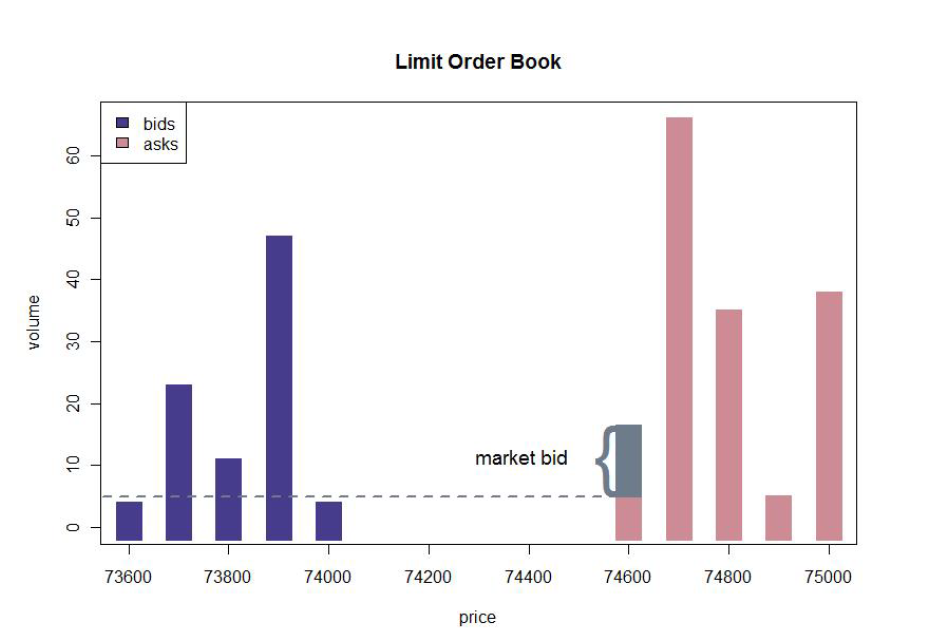
\includegraphics[width=0.9\textwidth]{chapters/chapter_trading_fund/figures/limitbk2.png} 
	   \caption{Limit Order Book---Marketable Bid. \label{fig:limbk2}}
	\end{figure}
	
When a market (or marketable) order is submitted, it decreases the number of outstanding orders at the opposite best price. For example, if a market bid order arrives, it will decrease the number of outstanding asks at the best price.
	\begin{figure}[!ht]
	   \centering
	   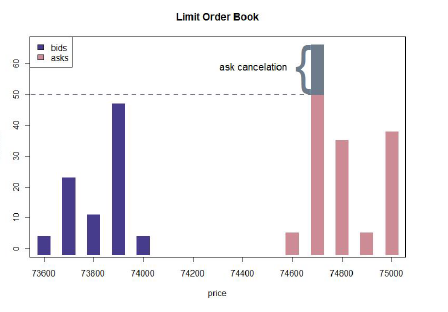
\includegraphics[width=0.9\textwidth]{chapters/chapter_trading_fund/figures/limitbk3.png} 
	   \caption{Limit Order Book---Ask Cancellation. \label{fig:limbk3}}
	\end{figure}
All unexecuted limit orders can be cancelled. When a cancellation occurs, it will decrease the number of outstanding orders at the specified price level. \\


Limit orders make up a significant percentage (70\%) of stock market trading activity. The main advantage of a limit order is that there is no price risk associated to it, that is when the order is executed the limit price is the maximum (for a buy order) or minimum (for a sell order) price that will be achieved. But if the limit order is not marketable, the execution is not guaranteed and the time to get an order executed depends on various market factors. 
The trade off between limit orders and marketable orders depends on the investors need for immediate liquidity and the fill probability of limit orders. The limit price chosen (how deep in the order book is the order placed) as well as the amount of liquidity ahead of the submitted order (how many shares will need to trade before the order gets executed following, for instance, a price/time priority order matching of the exchange) affect both the order fill probability as well as its expected time to fill. These two metrics are of particular relevance for execution algorithms and will be studied in more depth later. 
The execution of limit orders does affect how the quotes are posted and are updated.  
If the size of a market order exceeds the number of shares available at the top of book, it is usually split and is executed at consecutive order book levels until the order is filled. Market orders are usually restricted to be filled within a day and order placed after the markets close might be entered the next day. 
While we mostly considered limit and market orders, it is worth mentioning there exist a wide variety of orders types offered by different exchanges to facilitates certain types of trading activities. Two additional common order types are stop-limit orders and trailing stop orders. The former type is typically used to trade a security at a specified limit price once it traded through a given stop price. If the stock declines in value and trades below or at the stop price, the order will become a limit order rather than a market order. Trailing stop orders follow a similar objective but the stop price trails the best bid or ask by a certain percentage. These order types are primarily used by traders as a protection against sudden adverse market moves. \\

In addition to conditions on price, it is possible to add conditions on the life duration of the order known as Time-in-Force (TIF). The most common types of TIF instructions include Day orders which are valid for the full duration of the trading session and Good-Till-Cancel (GTC) orders which will be placed again on the exchange the next day with similar instructions if they were not fully filled. More sophisticated market participants aiming at achieving greater control over their executions tend to also favor Immediate-or-Cancel (IOC) and Fill-or-Kill (FOK) Time-in-Force instructions. An IOC order will get immediately cancelled back to the sender after reaching the matching engine if it doesn't get immediately a fill, and , in case of a partial fill, the unfilled portion of will also be cancelled, thus preventing it from creating a new price level in the order book. In a Fill-or-Kill scenario, the order gets either filled in its entirety or doesn't get filled at all. This instruction is particularly popular with high frequency market makers and arbitrageurs for which partial fills might result in unwanted legging risk as discussed in the Pairs Trading chapter. \\

Finally, it worth mentioning that some exchanges as well as alternative venues offer the ability of specifying minimum fill sizes whereby a limit order which might be eligible for a fill due to an incoming order at the same price level only receives a fill if the incoming order is larger than a pre-specified number of shares or notional value. This type of instruction is used by market participants as a way of minimizing the number of small fills which carry the risk of excessive information dissemination, in particular in dark pools where they can be used to detect the presence of larger limit orders that would otherwise not be visible to market participants.  

\subsection{How Double Auction Markets Work}

The term double auction refers to the nature of the markets where, unlike a common auction with one auctioneer and many potential buyers, there are multiple buyers and multiple sellers.



\subsubsection{Order Types}

The diversity of order types is a key component of continuous double auction electronic markets. Order types allow participants to precisely express their intentions with regards to interaction with the limit order book. Over time, in an effort to cater to sophisticated electronic traders, exchanges around the world have raced to offer ever more complex order types. Here, we will just provide a brief description of the vanilla ones:

\begin{itemize}
\item  Market: request to buy or sell immediately at the best available price. While it does not guarantee the trader a price, it guarantees execution. For small order sizes in actively traded names, a buy market order would execute close to the ask price, and a sell order close to the bid price.
\item  Limit: specify a maximum (resp. minimum) price at which the trader is willing to buy (resp. sell). If liquidity is available at a better price, the order will execute at that price.
\item  Peg: specify a price level at which the order should be continuously automatically repriced. For instance, an order pegged to the bid price will be automatically repriced as a higher price limit order each time the market bid price ticks up. This order type is particularly used for midpoint executions in non-displayed markets.
\item  Iceberg: limit order with a specified display quantity. In order to prevent information leakage to other market participants, a trader desiring to buy or sell a large quantity at a given price might elect to use an iceberg order with a small display size. For instance, for an order to buy 100,000 shares at \$20.00 with a display size of 2,000 shares, only 2,000 shares would be displayed in the order book. Once that quantity is executed, the order would automatically reload another 2,000 shares at \$20.00, and so on until the full quantity is executed.
\item  Hidden: while they are available to trade, these orders are not directly visible to other market participants in the central limit order book. 
\item  Stop: these orders are also not visible, but additionally are not immediately entered in the limit order book. They only become active once a certain price (known as the Stop Price) is reached or passed, then enter the order book as either limit or market order depending on the user setup.
\item  Trailing stop: these orders function like stop orders, but the stop price is dynamic rather than static (for instance: -3\% from previous close).

\item  AON (All-or-None): specifically request a full execution of the order. If the order is for 1500 shares but only 1000 are being offered, it won't be executed until the full quantity is available.

\item  OO (On-Open): specifically request an execution at the open price. It can be limit-on-open (LOO) or market-on-open (MOO).
\item  OC (On-Close): specifically request an execution at the close price. It can be limit-on-close (LOC) or market-on-close (MOC).
\item  IO (Imbalance only): provide liquidity intended to offset on-open/on-close orders imbalances during the Opening/Closing Cross. These generally must be limit orders.
\item  d-Quote: special order type on the NYSE mainly used during the close auction period.
\item  Funari: special order type on the Tokyo Stock Exchange which allows limit orders placed in the book during the continuous session to automatically enter the closing auction as market orders.
\end{itemize} 




\subsubsection{The Open Auction}

The Open Auction is only one of the types of call auctions that are commonly held on exchanges. The term "call auction" explains the liquidity aggregation nature of this event. Market participants are 'called' to submit their quotes to the market place, at a consistent time, in order to determine a matching price that will maximize the amount of shares that can be transacted. \\

To facilitate timely and orderly cross, auctions have strict order submission rules, including prescribed timing for entries (see Table~\ref{tab:NASDAQopen}) and information dissemination to prevent wild price fluctuations and ensure efficient price discovery. \\

% Requires the booktabs if the memoir class is not being used
\begin{table}[!ht]
   \centering
   \caption{Nasdaq Opening Cross\label{tab:NASDAQopen}}
   \hspace*{-0.8cm}
   \begin{tabular}{cc} 
	4:00 a.m. EST & Extended hours trading and order entry begins  \\ \hline
	9:25 a.m. EST & Nasdaq enters quotes for participants with no open interest \\ \hline
	9:28 a.m. EST & Dissemination of order imbalance information every 5 sec  \\ 
	 & Market-on-open orders must be received prior to 9:28 a.m.   \\ \hline	
	9:30 a.m. EST & The opening cross occurs		
   \end{tabular}
\end{table}	


Most exchanges publish order imbalance that exists among orders on the opening or closing books, along with the indicative opening or closing price and volume. For instance Nasdaq publishes the following information\footnote{Source: Nasdaq Trader website} between 9:28 a.m. EST and 9:30 a.m. EST,  every 5 seconds, on its market data feeds:
\begin{itemize}
\item  Current Reference Price: price within the Nasdaq Inside at which paired shares are maximized, the imbalance is minimized and the distance from the bid-ask midpoint is minimized, in that order.
\item  Near Indicative Clearing Price: The crossing price at which orders in the Nasdaq opening / closing book and continuous book would clear against each other. 
\item  Far Indicative Clearing Price: The crossing price at which orders in the Nasdaq opening / closing book would clear against each other. 
\item  Number of Paired Shares: The number of on-open or on-close shares that Nasdaq is able to pair off at the current reference price. 
\item  Imbalance Shares: The number of opening or closing shares that would remain unexecuted at the current reference price. 
\item  Imbalance Side: The side of the imbalance: B = buy-side imbalance; S = sell-side imbalance; N = no imbalance; O = no marketable on-open or on-close orders.
\end{itemize}



In a double auction setup, the existence of multiple buyers and sellers requires employing a matching algorithm to determine the actual opening price which we will illustrate with a practical example. Table~\ref{tab:openAuct} gives an example of order book submissions for a theoretical stock, where orders are ranked based on their arrival time.\\

Different exchanges around the world apply slightly different mechanisms to their auctions, but generally the following rules apply to match supply and demand:

\begin{itemize}
\item  The crossing price must maximize the volume transacted.
\item  If several prices result in similar volume transacted, the crossing price is the one the closest from the last price. 
\item  The crossing price is identical for all orders executed.
\item  If two orders are submitted at the same price, the order submitted first has priority over the other one.
\item  It is possible for an order to be partially executed if the other side quantity is not sufficient.
\item  "At Market" orders are executed against each others at the determined crossing price, up to the matching available quantity on both sides, but generally do not participate in the price formation process.
\item  For the Open Auction, unmatched "At Market" orders are entered into the continuous session Limit Order Book as limit orders at the crossing price.
\end{itemize} 



% Requires the booktabs if the memoir class is not being used
\begin{table}[!ht]
   \centering
   \caption{Pre-Open Order Book Submissions\label{tab:openAuct}}
   \hspace*{-2.0cm}
   \begin{tabular}{ccccc} 
	Timestamp & Seq. Number & Side & Quantity & Price \\ \hline
	9:01:21 & 1  &  B & 1500 &  12.10 \\
	9:02:36 & 2  &  S & 1750 & 12.12 \\	
	9:05:17 & 3  &  B & 4500  & 12.17 \\	
	9:06:22 & 4  &  S & 1750 & 12.22 \\
	9:06:59 & 5  &  S & 2500 & 12.11 \\	
	9:07:33 & 6 &  B & 1200 & 12.23 \\	
	9:07:42 & 7  &  B & 500 & 12.33 \\	
	9:08:18 & 8 &  B & 500 & 12.25 \\	
	9:09:54 & 9 &  S & 1930 & 12.30 \\	
	9:09:55 & 10 & B & 1000 & 12.21 \\	
	9:10:04 & 11 & S & 3500 & 12.05 \\	
	9:10:39 & 12 & B & 2000 & 12.34 \\	
	9:11:13 & 13 &  S & 4750 & 12.25 \\	
	9:11:46 &  14 & B  & 2750 & 12.19 \\	
	9:12:21 &  15 & S  & 10000 & 12.33 \\	
	9:12:48 &  16 & B  & 3000 & 12.28 \\	
	9:13:12 &  17 & B  & 5500 & 12.35 \\
	9:14:51 &  18 & S & 1800 & 12.18 \\
	9:15:02 &  19 & B & 800 & 12.17 \\
	9:15:37 &  20 & S & 1200 & 12.19 \\
	9:16:42 &  21 & S & 5000 & 12.16 \\
	9:17:11 &  22 & B & 12500 & 12.15 \\
	9:18:27 &  23 & S & 450 & 12.23 \\
	9:19:13 &  24 & S & 3500 & 12.20 \\	
	9:19:54 &  25 & B & 1120 & 12.16
   \end{tabular}
\end{table}

The first step is to organize orders by limit price, segregating buys and sells as shown in Table \ref{tab:openAuct2}. A buy order submitted with a limit price of 12.25 represents an intent to execute at any price lower or equal to 12.25. Similarly, a sell order submitted at 12.25 represents an intent to sell at any price higher or equal to 12.25. For each price level, we can then determine the cumulative buy interest and sell interest. The theoretical cross quantity at each price point is then simply the minimum of the cumulative buy interest and the cumulative sell interest as shown in Table \ref{tab:openAuct3}. The crossing price is determined as the price that would maximize the crossed quantity. In our example, the opening price will be 12.19, and the opening quantity will be 15,750 shares. \\

% Requires the booktabs if the memoir class is not being used
\begin{table}[!ht]
   \centering
   \caption{Ranked Order Book Submissions\label{tab:openAuct2}}
   \hspace*{-0.3cm}
   \begin{tabular}{cccccc} 
	Timestamp & Seq. Number & Buy Price & Buy Quantity & Sell Quantity & Sell Price\\ \hline
	9:13:12 &  17 & 12.35  & 5500 &  &\\
	9:10:39 & 12 & 12.34 & 2000 & & \\	
	9:07:42 & 7  &  12.33 & 500 &  &\\	
	9:12:21 &  15 & &  & 10000 & 12.33 \\	
	9:09:54 & 9 &  & & 1930 & 12.30 \\					
	9:12:48 &  16 & 12.28  & 3000 &  &\\	
	9:08:18 & 8 &  12.25 & 500 & & \\	
	9:11:13 & 13 &  & & 4750 & 12.25 \\	
	9:07:33 & 6 &  12.23 & 1200 & & \\		
	9:18:27 &  23 & & & 450 & 12.23 \\
	9:06:22 & 4  &  & & 1750 & 12.22 \\	
	9:09:55 & 10 & 12.21  & 1000 & &\\		
	9:19:13 &  24 & & & 3500 & 12.20 \\	
	9:11:46 &  14 & 12.19  & 2750 &  &\\		
	9:15:37 &  20 & & & 1200 & 12.19 \\
	9:14:51 &  18 & & & 1800 & 12.18 \\
	9:05:17 & 3  &  12.17 & 4500  & & \\		
	9:15:02 &  19 & 12.17 & 800 & & \\			
	9:16:42 &  21 & & & 5000 & 12.16 \\
	9:19:54 &  25 & 12.16 & 1120 & & \\		
	9:17:11 &  22 & 12.15 & 12500 & & \\
	9:02:36 & 2  &  & & 1750 & 12.12 \\		
	9:06:59 & 5  &  & & 2500 & 12.11 \\				
	9:01:21 & 1  &  12.10 & 1500 & &  \\
	9:10:04 & 11 & & & 3500 & 12.05 					
   \end{tabular}
\end{table}



% Requires the booktabs if the memoir class is not being used
\begin{table}[!ht]
   \centering
   \caption{Cumulative Order Book Quantities\label{tab:openAuct3}}
   \hspace*{-1.5cm}
   \begin{tabular}{ccccccc} 
	Price & Seq. Number & Cum. Buy Qty & Buy Qty & Sell Qty & Cum. Sell Qty & Qty Crossed at Price \\ \hline
	12.35 &  17 & 5500  & 5500 &  & 38130 & 5500\\
	12.34 & 12 & 7500 & 2000 & & 38130 & 7500\\	
	12.33 & 7  &  8000 & 500 &  & 38130 & 8000\\	
	12.33 &  15 & 8000 &  & 10000 & 38130 & 8000 \\	
	12.30 & 9 & 8000 & & 1930 & 28130 & 8000 \\					
	12.28 &  16 & 11000  & 3000 &  & 26200 & 11000\\	
	12.25 & 8 &  11500 & 500 & & 26200 & 11500\\	
	12.25 & 13 & 11500 & & 4750 & 26200 & 11500 \\	
	12.23 & 6 &  12700 & 1200 & & 21450 & 12700\\		
	12.23 &  23 & 12700 & & 450 & 21450 & 12700 \\
	12.22 & 4  & 12700 & & 1750 & 21000 & 12700 \\	
	12.21  & 10 & 13700  & 1000 & & 19250 & 13700\\		
	12.20 &  24 & 13700 & & 3500 & 19250 & 13700 \\	
	12.19 &  14 & 16450  & 2750 &  & 15750 & 15750\\		
	12.19 &  20 & 16450 & & 1200 & 15750 & 15750\\
	12.18 &  18 & 16450 & & 1800 & 14550 & 14550 \\
	12.17 & 3  &  20950 & 4500  & & 12750 & 12750\\		
	12.17 &  19 & 21750 & 800 & & 12750 & 12750\\			
	12.16 &  21 & 21750 & & 5000 & 12750 & 12750 \\
	12.16 &  25 & 22870 & 1120 & & 7750 & 7750\\		
	12.15  &  22 & 35370 & 12500 & & 7750 & 7750\\
	12.12  & 2  & 35370 & & 1750 & 7750 & 7750 \\		
	12.11  & 5  & 35370 & & 2500 & 6000 & 6000 \\				
	12.10 & 1  &  36870 & 1500 & & 3500 & 3500 \\
	12.05  & 11 & 36870 & & 3500 & 3500 & 3500 	

   \end{tabular}
\end{table}

The list of buy orders executed during the auction is shown in Table \ref{tab:openAuct4} and the sell orders in Table \ref{tab:openAuct5}. \\

% Requires the booktabs if the memoir class is not being used
\begin{table}[!ht]
   \centering
   \caption{Crossed Buy Orders\label{tab:openAuct4}}
   \hspace*{-3.3cm}
   \begin{tabular}{ccc} 
	Price & Seq. Number & Buy Qty  \\ \hline
	12.35 &  17 & 5500 \\
	12.34 & 12 & 2000\\	
	12.33 & 7  & 500\\			
	12.28 &  16 & 3000\\	
	12.25 & 8 & 500\\	
	12.23 & 6 & 1200\\		
	12.21  & 10& 1000\\		
	12.19 &  14  & 2050 		
   \end{tabular}
\begin{minipage}[t]{1\textwidth}
\small{*Order number 14 was for 2750 shares but did not get fully executed as the bid quantity up to 12.19 exceeded the offered quantity at that price. The balance of order 14 will then be posted as a limit order in the continuous trading session}
\end{minipage}   
\end{table}

	
% Requires the booktabs if the memoir class is not being used
\begin{table}[!ht]
   \centering
   \caption{Crossed Sell Orders\label{tab:openAuct5}}
   \hspace*{-3.3cm}
   \begin{tabular}{ccc} 
	Price & Seq. Number & Sell Qty  \\ \hline
	12.19 &  20 & 1200\\
	12.18 &  18 & 1800\\
	12.16 &  21 & 5000\\
	12.12  & 2  & 1750 \\		
	12.11  & 5  & 2500\\				
	12.05  & 11 & 3500 		
   \end{tabular}
\end{table}	




It is worth mentioning that the open auction tends to be considered as a major price discovery mechanism given the fact it occurs after a period of market inactivity when market participants were unable to transact. All new information accumulated overnight will be reflected in the first print of the day, matching buying and selling interests.  

As market participants with better information are more likely to be participating in the open auction with more aggressive orders in order to extract liquidity (and, as such, setting the price), the price discovery mechanism is often considered to be quite volatile and more suited for short-term alpha investors. Similarly, the period immediately following the open auction also tends to be much more volatile than the rest of the day. As a result of which, most markets experience wider spreads while market makers try to protect themselves against information asymmetry by quoting wider bid and offers. 
The increased volatility and wider spreads might discourage certain investors from participating in the market at the open auction and in the period immediately following the open. While this appears to be a reasonable idea from a price risk perspective, it is worth mentioning that for a lot of less liquid stocks (in particular small and mid cap stocks), the open auction can be a significant liquidity aggregation point that even surpasses the close auction. In Australia for instance, the bottom 50\% less liquid stocks have more volume trade in the open auction than in the close auction. Similarly, in Japan, the less liquid names see more volume trade in the open auction, but also in the afternoon open auction that follows the market lunch break.\\

From a pure execution standpoint, though, the usage of the open auction has to be considered carefully. While this represents a liquidity opportunity, the first print of the day can also have a significant anchoring effect on the stock price for the remainder of the day. So, participating in the open should be considered in light of the liquidity demand of the order: orders that are small enough can likely do without participating in the open auction and the continuous period immediately following; while large orders trying to extract significant liquidity from the market might likely benefit from participating in the open auction.


\subsubsection{Continuous Trading}

THE BORING PART .... INSERT ACTUAL MECHANICS \\


\subsubsection{The Closing Auction}

The Closing Auction tends to be the most popular of the call auctions for a variety of interesting reasons. Firstly, it is the last opportunity (exception made of off-hours trading) when market participants can transact in a relatively liquid environment before being exposed to the overnight period (when new information accumulates, but trades cannot easily take place). Secondly, with the increase in passive investment strategies providing investors with replication of a predetermined benchmark, the closing auction has become a particularly relevant price setting event (most passive funds NAV is based on close prices of the underlying assets). 

For such reasons, the closing auction is particularly important to many investors. From an execution standpoint, it is a major liquidity event that needs to be considered carefully. \\

INSERT ACTUAL MECHANICS \\

A large number of Quant and CTA funds are building their investment strategies using daily returns, essentially using the close price as a reference price for their investment decisions. Once their backtesting is built on close price data, they aim at obtaining an execution price equal to - or better than - the close price when implementing their strategies. 

It also represents a liquidity opportunity for active and passive investors to exchange large amounts of shares. As index constituents get updated on a regular basis (additions, deletions, weight increase/decrease) passive investors need to update their holdings to reflect the optimal composition of the benchmark they track and, in order to minimize their tracking error risk, that update needs to happen as close as possible to the actual update of the underlying benchmark. Consequently, most passive indexers tend to rebalance their portfolios on the same day the underlying index constituents are updated, using the close auction as a reference price, and resulting in significant flows at the close auction. Consequently, active investors looking to build a significant position (or unwinding one) can use these index events as a way of transacting a large amount of shares with low market impact at the close by being a liquidity providers to passive indexers.  



\subsection{Market Data}

Historical market data available to researchers and practitioners alike varied in degrees of granularity over time. From daily trade data (closing price and volume), to tick-by-tick trade and quote data (also known as TAQ data), to full message data, the progressive increase in granularity not only reflects the increase in intraday trading complexity but also opens up the way for more advanced strategies. \\

Initially researchers studying the dynamic of LOB had to be content with Trades and Quotes (TAQ) data which provide a time-stamped sequence of trades (Market Orders) and updates in the price and depth of bid and ask quotes. No other information beyond the best bid and the best offer are made available. Moreover, the updates contain changes at the two quotes and were aggregated. The aggregation was clearly a limiting factor as one could not discern the kind of events that led to the changing status of the book. The level II data that became available is a time-stamped sequence of trades and quotes for the top 5-levels of the LOB. This data is little deeper than TAQ data, but was still in aggregated form. But recently made available level III data contains time-stamped sequence of all (except for hidden orders) events that occur in the LOB. Every order is identified by a unique order-id and thus it can be tracked through its lifetime. \\



\subsubsection{Reference Data}

While often overlooked, or merely considered as an after thought in the development of a research platform, reliable reference data is the key foundation of a robust quantitative strategy development.

Commonly used reference data falls into different categories:

\begin{itemize}
\item \textbf{Symbology Mapping:} ISIN, SEDOL, RIC, Bloomberg Tickers, ... 

Quantitative strategies often leverage data from a variety of sources. Different providers key their data with different instrument identifiers depending on asset class or regional conventions, or sometime use their own proprietary identifiers (e.g. Reuter Identification Code - RIC, Bloomberg Ticker), therefore making symbology mapping the first step in any data join exercise. Such data is not static, one of the symbols can change on a given day and others remain unchanged for some time, complicating historical data joins even more.

It is important to note that such mapping needs to be persisted as point-in-time data and allow for historical "as of date" usage. Over the course of time, some instruments undergo ticker changes (for example from ABC to EDF on date $T_0$) without necessarily any particular change on the underlying asset. In such cases, market data recorded day-by-day in a trade database will change from being keyed on ABC to being keyed on EDF after the ticker change date $T_0$. This has large implications for practitioners working on datasets to build and backtest quantitative strategies. The symbology mapping should allow both backward and forward handling of the changes.

For instance, in the simple example mentioned, in order to efficiently backtest strategies over a period of time spanning $T_0$, one needs a robust mapping that will allow to seamlessly query the data for the underlying asset in a variety of scenarios such as:

\begin{itemize}
\item Signal generation: 30-day backward close time series as of date T < $T_0$:

{\tt select close from data where date in [T-30,  T], sym=ABC}

\item Signal generation: 30-day backward close time series as of date T = $T_0$+10:

{\tt select close from data where date in [$T_0$-20,  $T_0$+10], sym=EDF}

\item Position holding: 30-day forward close time series as of date T = $T_0$-10

{\tt select close from data where date in [$T_0$-10,  $T_0$+20], sym=ABC}

\end{itemize}

\item \textbf{Ticker Changes:} 

For comparable reasons as the ones described above in the Symbology Mapping section, one needs to maintain a historical table of ticker changes allowing to seamlessly go up and down time series. 


\item \textbf{Corporate Actions Calendars:} stock and cash dividends (both announcement date and ex date), stock splits, reverse splits, rights offer, mergers and acquisitions, spin off, free float or shares outstanding adjustments, quotation suspension.

Corporate actions impact the continuity of price and volume time series and, as such, need to be recorded in order to produce adjusted time series. The most common events are dividend distributions. On the day the dividend is paid, the corresponding amount is removed from the stock price, creating a jump in the price time series. The announcement date might also see the stock experience added volatility as investors react to the news. Consequently, recording these events proves to be valuable in the design of quantitative strategies as one can assess the effect on performance of dividends announcement or payment, and decide to either not hold a security that has an upcoming dividend announcement or, conversely, to build strategies that look to benefit from the added volatility. 

Additional types of corporate actions generating discontinuity in historical time series are stock splits or reverse splits and right offers. When the price of a stock becomes either too low or too high, a company might seek to split it to bring the price back to a level that is more conducive to liquid trading on exchanges\footnote{A very low price creates trading frictions as the minimum price increment might represent a large cost relative to the stock price. A very high price might also deter retail investors from investing into a security as it requires them to deploy too much capital per unit.}. When a stock experiences a 2:1 split, everything else being equal, its price will be halved and its volume will double. In order to prevent the time series to show a 50\% drop in price, all historical data will then need to be adjusted backward to reflect the split.

Mergers \& Acquisitions and Spin-offs are also regular events in the lifecycle of corporations. Their history needs to be recorded in order to account for the resulting changes in valuation that might affect a given ticker or tickers. These situations can also be exploited by trading strategies known as Merger Arbitrage.

Stocks quotation can be suspended as a cooling mechanism (often at the request of the underlying company) to prevent excess price volatility when significant information is about to be released to the market. Depending on the situation, the suspension can be temporary and intraday, or can last for extended periods of time if the market place allows it\footnote{For instance, it was the case for a large number of companies in China in 2016.}. Suspensions result in gaps in time series and are worth keeping track of as they can impact strategies backtesting (inability to to enter or exit a position, uncertainty in the pricing of composite assets if a given stock has a significant weight in ETFs or Indexes). 
Some markets will also suspend trading if the price swings more than a predefined amount (limit up / limit down situations) for either a period of time or for the remainder of the trading session.

\item \textbf{Static Data:} country, sector, primary exchange, currency and quote factor.

Pure static data is also relevant for the development of quantitative trading strategies. In particular, country, currency and sector are useful to group instruments based on their fundamental similarities. A well known example is the usage of sectors to group stocks in order to create pairs trading strategies. It is worth mentioning that there exist different types of sector classifications (e.g. GICS\textsuperscript\textregistered from S\&P, ICB\textsuperscript\textregistered from FTSE) offering several levels of granularity\footnote{The Global Industry Classification Standard (GICS) structure consists of 11 sectors, 24 industry groups, 68 industries and 157 sub-industries. An example of this hierarchical structure would be: Industrials / Capital Goods / Machinery / Agricultural \& Farm Machinery.}, and that different classifications might be better suited to different asset classes or countries. The constituents of the Japanese index TOPIX, for instance, are classified into 33 sectors that are thought to better reflect the fundamental structure of the Japanese economy and the existence of large diversified conglomerates. 

Maintaining a table of the quotation currency per instrument is also necessary in order to be able to aggregate positions at a portfolio level. Some exchanges allow the quotation of prices in currencies different from the one of the country in which the exchange is located \footnote{For example, Jardine Matheson Holdings quotes in USD on the Singapore exchange while most of the other securities quote in Singapore Dollars.}. Additionally, the Quote Factor associated with the quotation currency time series needs to be stored. To account for the wide range of currency values and preserve pricing precision, market data providers might be publishing FX rates with a factor of 100 or 1000. Hence, to convert prices to USD one needs to multiply by the quote factor: $usd price = local price * fx * quote factor$. Similarly, some exchanges quote prices in cents, and the associated quotation currency is reflected with a small cap letter: GBP/GBp, ZAR/ZAr, ILS/ILs, ...).

\item \textbf{Exchange Specific Data:}  

Despite the electronification of markets, individual exchanges present a variety of differences that need to be accounted for when trading strategies. The first group of information concerns the hours and dates of operation:

\begin{itemize}
\item Holiday calendar: as not all exchanges are closed on the same day, and trading days off do not always fully follow the country public holidays, it is valuable to record them in particular in an international context. Strategies trading simultaneously in several markets might not perform as expected if one of the markets is closed while the others are open. Similarly, execution strategies in one market might be impacted by the absence of trading in another market (for instance, European equities markets volume tends to be 30\% to 40\% lower during U.S. market holidays).
\item Exchange sessions hours: 

Exchange session hours, auction times as well as their respective cut-offs for order submission, lunch break hours, 
F\&O Sessions and end of trading vs. settlement time

In Indonesia, for instance, markets have different trading hours on Fridays. Monday through Thursday the Indonesia Stock Exchange (IDX) is open from 9:00 AM to 12:00 PM, and then, from 1:30 PM to 4:00 PM. On Fridays, however, the lunch break is one hour longer and stretches from 11:30 AM to 2:00 PM. This weekly seasonality effect is particularly important to consider when building volume profiles as described in the next chapter.
Along with local times of operation, it is necessary to consider eventual Daylight Saving Time (DST) adjustments that might effect the relative trading hours of different markets (some countries do not have DST adjustment at all, while for countries that do have one, the dates at which it applies are not always coordinated). Usually, DST starts about two weeks prior to its start in Europe, bringing the time difference between New York and London to 4 hours instead of 5 hours. This results in the volume spike in European equities associated to the U.S. market open being one hour earlier, requiring adjustment of volume profiles used for trading execution.
Some exchanges might also adjust the length of trading hours during the course of the year. In Brazil for instance, the Bovespa trading hours are 10:00 AM to 6:00 PM from October to March, but an hour shorter (10:00 AM to 5:00 PM) from April to September to be more consistent with U.S. market hours.
Finally, within one country there might also exist different trading hours by venues as it is the case in Japan where the Nagoya Stock Exchange closes 30 minutes after the major Tokyo Stock Exchange.
\item Disrupted days: exchanges outages or trading disruptions, as well as market data issues, need to be recorded so they can be filtered out when building or testing strategies as the difference in liquidity patterns or the lack of data quality might impact the overall outcome.

\end{itemize}

Additionally, exchanges also have specific rules governing the mechanics of trading, such as:
\begin{itemize}
\item Tick Size: 
\item Trade and Quote lots:
\item Limit-up and Limit-down constraints:
\item Short Sell restrictions
\end{itemize}

\item \textbf{Market Data Condition Codes:} 

With ever-growing market microstructure complexity, market data dissemination has grown proportionally complex as well. While it is possible to store daily data as a single entry per day and per instrument, investors building intraday strategies likely need to collect tick by tick data of all the events occurring in the market place. To help classify events, exchanges and market data providers attribute so-called condition codes to the trades and quotes they publish. These condition codes vary per exchange and per asset class, and each market event can be attributed several codes at once. So, to aggregate intraday market data properly and efficiently, and decide which events to keep and which ones to exclude, it is necessary to build a mapping table of these condition codes and their meaning: auction trade, lit or dark trade, cancelled or corrected trade, regular trade, off-exchange trade reporting, block-size trade, trade originating from a multi-leg order such as an option spread trade, ... 

For instance, in order to assess accessible liquidity for a trading algorithm, trades that are published for reporting purposes (e.g. negotiated transactions that happened off-exchange) need to be excluded. These trades should also not been used to update some of the aggregated daily data used in the construction of trading strategies (daily volume, high, low, ...). Execution algorithms also leverage extensively intraday liquidity distribution metrics to gauge their own participation in auctions and continuous sessions, or in lit versus dark venues, therefore requiring a precise classification of intraday market data. 

\item \textbf{Special Day Calendars:} 

Over the course of a year, certain days present liquidity characteristics that need to be accounted for in both execution strategies or alpha generation. Here too, the diversity of events across markets and asset classes can be quite challenging to handle. Among the irregular events that affect liquidity in equities markets and need to be accounted for, we can mention the following non-exhaustive list for illustration purposes: half trading days following Christmas and Thanksgiving in the U.S. or on the Ramadan eve in Turkey; Taiwanese market opening on the weekend to make up for lost trading days during holiday periods; Korean market changing its trading hours on the day of the nationwide university entrance exam; Brazilian market opening late on the day following the Carnival; etc. 

There are also special days that are more regular and easier to handle. The last trading days of the months and quarters, for instance, tend to see additional trading activity as investors rebalance their portfolios. Similarly, options and futures expiry days (quarterly/monthly expiry, 'Triple Witching'\footnote{Triple witching days happen four times a year on the third Friday of March, June, September and December. On these days, the contracts for stock index futures, stock index options and stock options expire concurrently.} in the U.S., Special Quotations in Japan, etc.) tend to also have relative excess trading volume and different intraday patterns resulting from hedging activity and portfolios adjustments. Consequently, they often need to be handled separately, in particular when modeling volume. As most execution strategies make use of relatively short interval volume metrics (e.g. 30-day or 60-day ADV), one single data point can be enough to impact the overall level inferred. Similarly autoregressive models of low order might underperform both on special days and on the days following them. As a result, modelers often opt for removing special days from datasets and model normal days first. Then, special days are modeled separately, either independently or using the normal days as a baseline. 

In order to reflect changes in the market and remain consistent with index inclusion rules, most indexes need to undergo regular updates of their constituents as well as their respective weights. Most of the significant indexes do so at regular intervals (annually, semi-annually or quarterly) on a pre-announced date. At the close of business of that day, some stocks might be added to the index while others are removed, or the weight of each stock in the index might be increased or decreased. These events, known as index rebalances, are particularly relevant to passive investors who are tracking the impacted index. In order for them to minimize the tracking error to their benchmark index, they need to also adjust their holdings accordingly. Additionally, as most funds are benchmarked at the close price, there is an incentive for fund managers to try to rebalance their holdings at a price as close as possible to the official close price of the day the index rebalance becomes effective. As a result, on these days, intraday volume distribution is significantly skewed toward the end of day and requires adjustment of execution strategies.

It is worth noting that a special day calendar usage needs not be limited to the country where the event occurs. On days when the U.S. Equities market is closed, there is usually also a significant drop in volume traded in European markets, so it is always valuable to investigate the cross sectional effect of special days.


\item \textbf{Futures-specific Reference Data:} 

Futures contracts present particular characteristics requiring additional reference data to be collected. One of the core differences of futures contracts compared to regular stocks is the fact that instruments have an expiry date, after which they cease to exist. For the purpose of backtesting strategies, it is necessary to know which contract was live at a point in time through the use of an expiry calendar, but also which contract was the most liquid (for instance, equity index futures tend to be the most liquid for the first contract available (also known as front month) while energy futures such as oil tend to be more liquid for the second contract. While this may appear to be trivial, when building a trading strategy and modeling prices time series, it is particularly important to know which contract carries the most significant price formation characteristics and what is the true liquidity available in order to estimate transaction costs such as market impact. 

The task of implementing a futures expiry calendar is further complicated by the fact there is no real standardized frequency that applies across markets. For instance, European equity index futures tend to expire monthly, while U.S. index futures expire quarterly. Some contracts even follow an irregular cycle through the course of the year as it is the case for grain futures (e.g. wheat) that were originally created for hedging purposes and as a result have expiry months that follow the crop cycle (GIVE AN EXAMPLE OF WHEAT FULL YEAR CYCLE).

The fact futures contracts expire on a regular basis has further implications in terms of liquidity. As investors holding these contracts might want to maintain their exposure for longer than the lifespan of the contract, they need to roll over their positions onto the next contract. There is often a noticeable difference in the liquidity of consecutive contracts (for instance, the front contract of the S\&P500 (e.g. ESM8) trades roughly 2 million contracts per day -- NEED TO CHECK ACTUAL ADV -- while the next month contract (ESH8) only trades 100,000 contracts per day --- NEED TO CHECK THE ACTUAL ADV --. However, this liquidity relationship will invert in the few days leading to the expiry of the front contract as most investors roll their positions, and the most liquid contract will become the back month contract (INSERT GRAPH). As a result, when computing rolling-window metrics (such as average daily volume for instance), it is necessary to account for potential roll dates that might have happen during the span of the time series. In the example above, a simple 60-day average daily volume on ESH8 taken in early April 2018 would capture a large number of days with very low volume (January-March) owing to the fact the most liquid contract at the time was the ESM8 contract, and not accurately represent the volume activity of the S\&P500 futures contract. A more appropriate average volume metric to be used as a forward looking value for execution purposes would blend the volume time series of ESH8 prior to the roll date, and ESM8 after the roll date\footnote{It is worth noting that different contracts 'roll' at different speed. While for monthly expiry contracts it is possible to see most of the open interest switch from the front month contract to the back month on the day prior to the expiry, for quarterly contracts it is not uncommon to see the roll happen over the course of a week or more, and the front month liquidity vanish several days ahead of the actual expiry. Careful modeling is recommended on a case by case basis.}. 

Additionally, in order to efficiently merge futures positions with other assets in an investment strategy, one needs to store reference data relative to the quotation of these contracts: contract size (translation between the quotation points and the actual monetary value), currency, etc. 

Finally, futures markets are characterized by the existence of different market phases during the day, with significantly different liquidity characteristics. For instance, equity index futures are much more liquid during the hours when the corresponding equities markets are open. However, one can trade during the overnight session if they need to. The overnight session being much less liquid, the expected execution cost tends to be higher, and as such, the various market data metrics (volume profile, average spread, average bid-ask sizes, ...) should be computed separately for each market phase, which requires maintaining a table of the start and end times of each session for each contracts. 

\item \textbf{Options-specific Reference Data:} Options chain

Similar to futures contracts, options contracts present a certain number of specificities for which reference data need to be collected. On top of the similar feature of having a particular expiry date, options contracts are also defined by their strike price. The combination of expiries and strikes is known as the the option chain for a given underlier. 

The ability to map equities tickers to options tickers and their respective strike and expiry date allows for the design of more complex investment and hedging strategies. For instance, distance to strike, change in open interest of puts and calls, open interest can all be used as signals for the underlying security price.

\item \textbf{Market-Moving News Releases:} 

Macro-economic announcements are known for their ability to move markets substantially. Consequently, it is necessary to maintain a calendar of their occurrences in order to assess their impact on strategies and decide how to best react to them. The most common ones are central banks announcements or meeting minutes releases of the major economies (FED/FOMC, ECB, BOE, BOJ, SNB), Non-Farm Payrolls, PMI, Crude Oil Inventories, etc.

While these news releases impact the broad market or some wide sectors, there are also stock specific releases that need to be tracked. 
Earning calendars (dates and times / backward and forward), specialized sector events such as FDA results for the healthcare and biotech sectors  .... (Dates and times / backward and forward)



\item Related tickers: Primary tickers to composite ticker mapping, dual listed/fungible securities in US and Canada, local and foreign boards in Thailand, 

\item \textbf{Composite Assets:} time series of constituents, time series of divisor (eg change in free float,...), time series of cash components, mapping to underlying ticker, 

\item \textbf{Latency tables:} routing, market data collection

This latest type of data would only be of interest for strategies and research in the higher frequency trading space. For these, it might be relevant to know the distribution of latency between different data centers as they can be used for more efficient order routing as well as reordering time series that might have been recorded in different locations.

\end{itemize}

While the points mentioned above represent a non exhaustive list of the reference data available to build a quantitative research platform, they highlight the challenges that need to be accounted for when designing and implementing algorithmic trading strategies. Once in place, a proper set of reference data will allow to harness the actual content of the following types of data.

\subsubsection{Fundamental Data}

\begin{itemize}
\item key ratios: EPS, P/E, P/B, ...
\item Analyst recommendations, consensus, price targets
\item Earnings consensus
\item Holders // check FINRA/SEC filing forms
\item Insiders Purchase/Sale // check FINRA/SEC filing forms
\end{itemize}

\subsubsection{Daily Statistics}

\begin{itemize}
\item Open, High, Low, Close (OHLC) / Prev Close Price and Date (for computation efficiency such as overnight gap: but needs careful 'adjust=True...), last before close Time/Price
\item Volume + lit/dark breakdown
\item VWAP
\item Short Interest / utilization / days-to-cover
\item Auctions volume (up to 4 of them, + liquidity / intraday ones)
\item Spread (avg, med, twavg) --> or better: parametrized distribution which can then be used in a Bayesian update setup
\item Number of trades
\item Trade size (avg, med) --> or better: parametrized distribution which can then be used in a Bayesian update setup
\item Number and frequency of quote updates 
\item Top of book size
\item Depth of book (price and size)
\item Ticking time (avg, med) --> or better: parametrized distribution which can then be used in a Bayesian update setup
\item Futures and Options:
\begin{itemize}
\item Open Interest
\item Greeks 
\item Implied Vol
\item Basis / dividends estimates
\item Fair Value
\end{itemize}

\item Index-level data for relative measures: OHLC, Overnight gap, ..., benchmark rates (repo, 2y, 10y, 30y?)
\item Asset Class Specific: FI, FX, Credit
\begin{itemize}
\item Yield
\item CDS Spread
\item Closed End Fund: premium / discount
\item USDollar Index
\end{itemize}

\end{itemize}

Can also include pre-computed aggregated X-day trailing data (essentially for computation efficiency in backtest), in particular for normalisation purposes (eg size as a percentage of ADV, spread in relation to long-term average, ...)
\begin{itemize}

\item X-day volatility
\item X-day ADV / Avg auction Volume
\item Beta (full, up-days/down-days) wrt index or sector
\item Correlation to reference index
\end{itemize}

--> Aggregated data need to fully support the peculiarities described in the Reference Data section (for instance: existence of special or event days which, if included, can significantly skew intraday distribution of values; mishandling of market asynchronicity resulting in inaccurate sensitivities computations such as beta or correlation)

\subsubsection{Bin Data}

Aggregated bar data....
Particularly useful to detect seasonalities eg Spread size shrinking in the post-open price discovery period and for quick backtesting of intraday trading strategies

\subsubsection{Level 1: Trade, Quotes, BBO and NBBO}

Superbook \\
Trade time, trade exch time, trade source time \\
Price, size, bid ask price size \\
Quote time, exch time, source time \\
Trade status \\
LULD indicator \\
Qualifiers TRADES AND QUOTES \\
Part ID

\subsubsection{Level 2: Market Depth}


\subsubsection{Level 3: Orders}

--> mention that for generalisation purposes we take the example of US Level 3 data, in particular w.r.t. Table 8.1  \\

\noindent\textbf{Description of Level III data:} The dataset consist of activities during the entire trading session, including early and late hours from 6:00~A.M. to 8:00~P.M. EST in a trading day. It provides intraday depth book activity for 12000 tickers from major national exchanges: Nasdaq, Direct Edge, NYSE, ARCA and BATS (exact number of exchanges depends on the historical period). All messages are consolidated into one file ordered by timestamp. This data allows to build a full national depth book at any moment intraday. The description of the level III data is given in Table~\ref{tab:level3data}. \\
	\begin{table}[!ht]
	\centering
	\begin{tabular}{lp{0.8\textwidth}} \hline
	Variable & Description \\
	& \\
	Timestamp: & Number of milliseconds after the midnight. \\
	& \\
	Ticker: & Equity symbol (up to 8 characters) \\
	& \\
	Order: & Unique order ID. \\
	& \\
	T & Message type. Allowed values: \newline \begin{minipage}[t]{0.6\textwidth} \begin{itemize} \item ``B''---Add buy order \item ``S''---Add sell order \item ``E''---Execute outstanding order in part \item ``C''---Cancel outstanding order in part \item ``F''---Execute outstanding order in full \item ``D''---Delete outstanding order in full \item ``X''---Bulk volume for the cross event \item ``T''---Execute non-displayed order \end{itemize} \end{minipage} \\
	& \\
	Shares & Order quantity for the ``B'', ``S'', ``E'', ``X'', ``C'', ``T'' messages. Zero for ``F'' and ``D'' messages. \\
	& \\
	Price & Order price, available for the ``B'', ``S'', ``X'' and ``T'' messages. \newline Zero for cancellations and executions. The last 4 digits are decimal digits. The decimal portion is padded on the right with zeros. The decimal point is implied by position; it does not appear inside the price field. Divide by 10000 to convert into currency value. \\ 
	& \\
	MPID & Market Participant ID associated with the transaction (4 characters) \\
	& \\
	MCID & Market Center Code (originating exchange---1 character) 
	\end{tabular}
	\caption{Level III data \label{tab:level3data}}
	\end{table}
	

\noindent\textbf{Special types of orders:} While the display and issuance of new ID to the modified order varies from exchange to exchange, we provide a brief description of these orders below:

\begin{enumerate}[1.]
\item Order subject to price sliding: the execution price could be one cent worse than the display price at NASDAQ; it is ranked at the locking price as a hidden order, and displayed at the price one minimum price variation (normally 1 cent) inferior to the locking price. New order ID will be used if the order is replaced as a display order. At other exchanges the old order ID will be used.

\item Pegged order: Based on NBBO, not routable, new timestamp upon re-pricing, display rules vary over exchanges.

\item Mid-point peg order: Non-displayed, can result in half-penny execution.

\item Reserve order: displayed size is ranked as a displayed limit order and the reserve size is behind non-displayed orders and pegged orders in priority. The minimum display quantity is 100 and this amount is replenished from the reserve size when it falls below 100 shares. A new timestamp is created and the displayed size will be re-ranked upon replenishing.

\item Discretionary order: displayed at one price while passively trading at a more aggressive discretionary price. The order becomes active when shares are available within the discretionary price range. Ranked last in priority. The execution price could be worse than the display price.

\item Intermarket sweep order: order that can be executed without the need of checking the prevailing NBBO.  
\end{enumerate}


Some key measures of the LOB are: relative position of an order from the top position of the side (buy or sell), the depth which is the total number of shares at a given price and the depth profile of the book reflects the depth of both prices. Large market orders can shift the bid and ask prices. If the limit price of a new order crosses the best price on the opposite side of the book, it is executed immediately and these are termed as crossing or marketable limit orders. These are used at times to explore the existence of hidden orders.


The limit order book data provides a rich source of information to better understand the market microstructure. The information is also useful for developing trading strategies. Some key issues that may be explored are:

\begin{itemize}
\item The pattern of inter-arrival times of various events.
\item Arrival and cancellation rates as a function of distance from nearest touch price.
\item Arrival and cancellation rates as a function of other available information, such as in the queue on either side of the book.
\end{itemize}

The key issues from the trading point of view are:

\begin{itemize}
\item What is the impact of market order on the limit order book?
\item What are the chances for a limit order to move up the queue from a given entry position?
\item What is the probability of making the spread?
\item What is the direction of the price movement in short duration?
\end{itemize}

\section{The Dynamics of Trading: Market Micro-structure}

Market structure constraints imposed on execution:

\begin{itemize}
\item tick sizes
\item Short sell rules
\item Long queue names
\item 10b-18 rule in US equity
\item Pro-rata markets
\end{itemize}

\section{Execution and its components}
\subsection{Benchmarks}

\begin{itemize}
\item Arrival
\item Inline
\item Full day or Period VWAP
\item Close
\item "All of the above" while completing as much as possible
\end{itemize}

Additional metrics considered for execution performance:
\begin{itemize}
\item completion rate
\item Make/take ratio
\item Mean vs Variance of performance...
\end{itemize}

The benchmark represents a quantitatively measurable observation of the execution objective, which needs to be translated into a series of actual trading actions which are described below


\subsection{Scheduling}

The Macro Trader --> ANSWERS THE QUESTION: How much should I trade in each period?

\begin{itemize}
\item Auctions: to partake or not to partake?
\item Spread Cost vs Liquidity Reward in the "price discovery" period post-open
\item Intraday volume patterns (see next chapter). The value of total day forecast vs intraday distribution?
\item Weekly seasonalities: Monday's are price discovery days, Wed are great?
\item Special days: index events and expiries, quoting deeper at times of news release, ...
\end{itemize}


\subsection{Order Placement (Lit and Dark)}

The Micro Trader --> ANSWERS THE QUESTION: At what price should I trade?

Lit and Dark order placements present different challenges. While lit executions are directly observable and can be observed in public market data feeds, dark executions tend to be reported in aggregate, thus making attribution of actual execution venue more challenging. For instance, if solely observed from market data, dark executions in the US cannot be directly attributed one of the non-displayed venues. However, if observed from the point of view of an executing entity (through execution fills received), one can obtain sensored observations of the available -- otherwise invisible -- liquidity (I.e. When receiving a fill for X shares one knows there was at least X shares available to trade on the other side).

\begin{itemize}
\item Lit Order Placement logic:

\item Dark Order Placement logic: the question one needs to answer here is: given X shares to execute and Y available venues, what is the combination of shares sent to different venues that maximizes the fill probability and minimizes the time to fill?

\end{itemize}


\subsection{Order Routing}

The Smart Order Router --> ANSWERS THE QUESTION: Where should I trade in a fragmented marketplace?

This is only a particular concern in markets that present a significant level of fragmentation, such as the US equity market. 

\begin{itemize}
\item Probability of Fill: how probable is it to get filled? 

\item Time to fill
\end{itemize}


\subsection{RFQ Markets}
What happens in other asset classes???